\documentclass[a4paper, 11pt]{article}
\usepackage[left=2.5cm,right=2.5cm,top=3cm,bottom=3cm,a4paper]{geometry}
\usepackage{kotex}
\usepackage{color}
\usepackage{enumitem}
\usepackage[cmyk, dvipsnames, svgnames]{xcolor}
\usepackage{graphicx}
\DeclareGraphicsExtensions{.pdf,.png,.jpg}



\title{\textbf{\Huge오목 한글 설명서}}
\author{\textbf{\LARGE5조}}
\begin{document}
	
	\maketitle
	
	\vspace{6cm}
	\begin{center}
		\textbf{\large20134824김민석}\\
		\textbf{\large20134852허정건}\\
		\textbf{\large20134867이현문}\\
	\end{center}
	
	
	
	
	\maketitle
	\newpage
	\thispagestyle{empty}        
	\mbox{}
	
	\begin{center} 
		\textbf{\Huge목차}\\
	\end{center}
	\vspace{1cm}
	\section{프로그램 선택 이유}
	\vspace{1cm}
	\section{프로그램 설명}
	\begin{itemize}
		\item 소개 및 목표
	\end{itemize}
	\vspace{0.5cm}
	\section{사용 설명}
		\begin{itemize}
		\item 규칙
		\item 조작법
	\end{itemize}
	\vspace{0.5cm}
	
	\section{기능 설명}
	\begin{enumerate}
		\item a설명
		\item b설명
		\item c설명
	\end{enumerate}
	
	
	
	
	\vspace{1cm}
	\section{버그와 개선할점}
	
	\vspace{1cm}
	\section{느낀점}
	
	
   \newpage
	\title{\textbf{\Huge1. 프로그램 선택 이유}}\\
	
	{\Large
	우선 수 많은 오픈소스중에 설명서를 만듦에 있어 평소 우리가 자주 사용하지 않는 프로그램 보다 더 익숙하고 쉽게 접근할 수 있는 프로그램을 찾아 설명서를 만들어 보자는 생각에서 부터 오픈소스를 찾게되었다.\\
	평소 게임을 좋아하는 우리 팀은 자연스럽게 게임에 대한 오픈소스를 찾게되었고 그로부터 우리나라의 전통놀이인 오목게임의 오픈소스를 찾게되었다. \\
	전통놀이 오목의 설명서를 만들면서 오목게임도 할 수 있고,설명서를 만들어 다른 사람에게 도움도 줄 수 있어 일석이조라고 생각하여 결국 이 프로그램을 선택하게 되었다.
	}\\\\\\\\


	\newpage
	\title{\textbf{\Huge2. 프로그램 설명}}\\
	\begin{itemize}
		\item \LARGE소개 
	\end{itemize}
	{\Large
	이 프로그램은 네이버 블로거 dnpc7848 의 개인 공부용도로 프로그램을 개발하였으며, 현재 모든 소스를 오픈하고 수정과 배포에 제한을 두지 않고 있다.\\
	}
	\begin{itemize}
		\item \LARGE목표
	\end{itemize}
	{\Large
	일반 룰, 고모쿠 룰, 렌주 룰 세 가지룰에 대해 각 룰을 설명하고,이 프로그램의 설명을 통해
	남녀노소 가리지 않고 누구나 쉽게 전통놀이 오목을 접하고 배울 수 있게 함에 목표를 둔다.
	}\\\\\\\\\\

 \begin{figure}[h] %%% t: top, b: bottom, h: here
	\begin{center}
		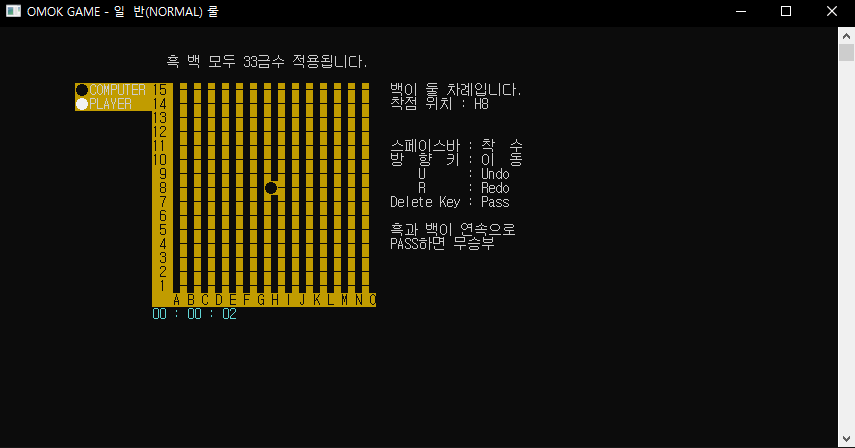
\includegraphics[width=1.0\linewidth]{intro.png}
	\end{center}
	\caption{intro}
	\label{fig:long}
	\label{fig:onecol}
\end{figure}

\end{document} 